\item \textbf{{[}HCI/PRELIM/9597/2019/P2/Q7{]} }

The algebraic expression \texttt{X = 2 {*} A + B} could be held in
a binary tree as:
\begin{center}
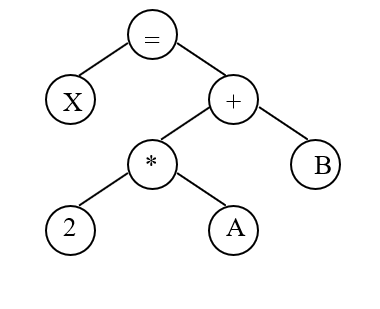
\includegraphics[width=0.5\paperwidth]{C:/Users/Admin/Desktop/Github/question_bank/LyX/static/img/9597-HCI-2019-P2-Q7}
\par\end{center}

This tree can then be read using the following algorithm:

process left subtree 

process right subtree 

read root node

This will give \texttt{X 2 A {*} B + =} which is the reverse Polish
form of the expression.
\begin{enumerate}
\item Using diagrams to help the explanation, or otherwise, show how a computer
can use a stack to evaluate the expression from its reverse Polish
form. \hfill{}{[}4{]}
\item The tree in the example could be stored in an array called TREE.
\noindent \begin{center}
\begin{tabular}{|c|c|c|c|}
\hline 
TREE{[}9{]} &  &  & \tabularnewline
\hline 
TREE{[}8{]} &  & -1 & \tabularnewline
\hline 
TREE{[}7{]} &  & 5 & \tabularnewline
\hline 
TREE{[}6{]} &  &  & \tabularnewline
\hline 
TREE{[}5{]} & 2 &  & \tabularnewline
\hline 
TREE{[}4{]} &  &  & \tabularnewline
\hline 
TREE{[}3{]} & X &  & \tabularnewline
\hline 
TREE{[}2{]} &  &  & \tabularnewline
\hline 
TREE{[}1{]} & B &  & \tabularnewline
\hline 
TREE{[}0{]} & = & 3 & 4\tabularnewline
\hline 
\end{tabular}
\par\end{center}

The values in each location in the array are: node value; left pointer;
right pointer. Where no left or right pointer exists the rouge value
-1 is used. Copy and complete the array for the example. (Note that,
since in the example there are only seven nodes, three rows of the
array will be unused.) \hfill{}{[}5{]}
\item Draw a tree similar to the one in the example which would represent
the expression:
\begin{center}
\texttt{Y = 2 {*} (A + B) \textendash{} (A \textasciicircum{} 2)} 
\par\end{center}

where \texttt{x \textasciicircum{} y} means $\mathtt{x^{y}}$.\hfill{}{[}3{]}
\item Using the algorithm in the example, and your tree, write out the reverse
Polish form of the expression in \textbf{part} (c). \hfill{}{[}3{]}
\end{enumerate}